\section{Client Usage}
\label{sec:client_usage}
The client can generally do three things; commit a problem, see status of his/her problems, or search the database for problems.
The first two are based on there corresponding use cases in section \ref{sec:usecase}.
The search function was added as a functionality for client because we assume that it would primarily be persons with a new problem who might want to search for others problems.

The following subsections describes the three usage of the system which the \aclient[] has access to.

\subsection{Commit a Problem}
\begin{figure}[htb]
	\centering
		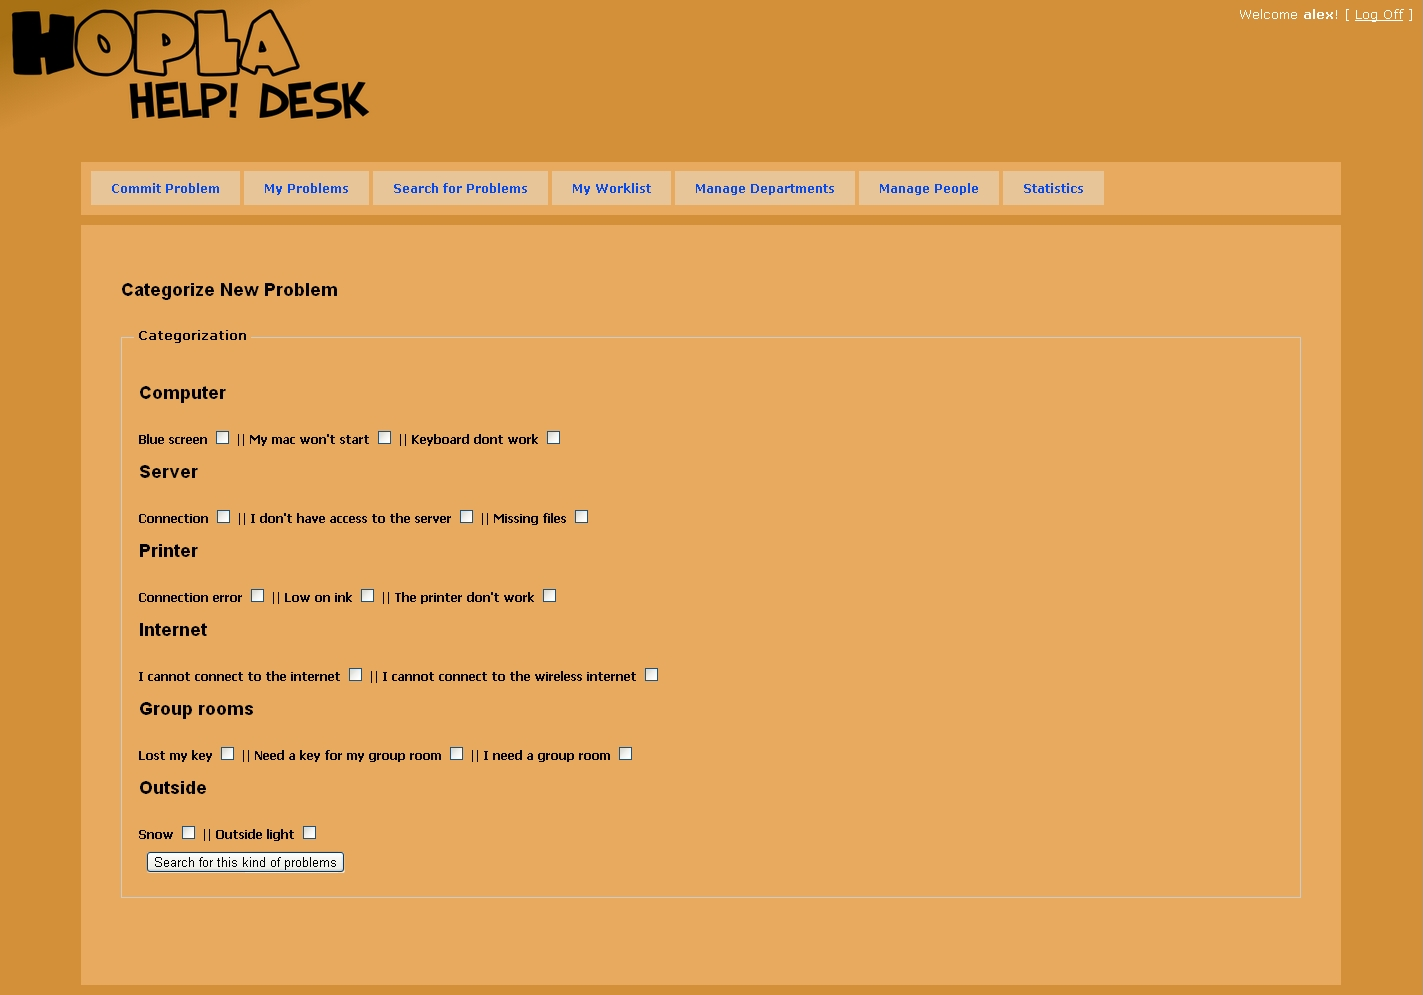
\includegraphics[width=1.00\textwidth, clip=true, trim=2.9cm 0.5cm 3cm 8cm]{input/implementation/program_presentation/commit.png}
	\morscaption{The categorization step in committing a problem}
	\label{fig:commit}
\end{figure}
The process of committing a problem starts with a click on the Commit Problem menu point, which can be seen in figure \ref{fig:master}.
When Commit Problem is clicked the user is asked to categorize the problem in the window showed in figure \ref{fig:commit}.
As the figure shows the tags, the check boxes, are ordered under headlines.
These headlines are categories.

When the problem is categorized the system searches for problems matching the specified tags, the search function is described in \ref{sec:search}.
The problems found in the search are listed in a table with columns showing number of matching tags, deadline, estimated time of completion, and title and description.
The last column also shows whether the given problem is solved or not.

\begin{figure}[htb]
	\centering
		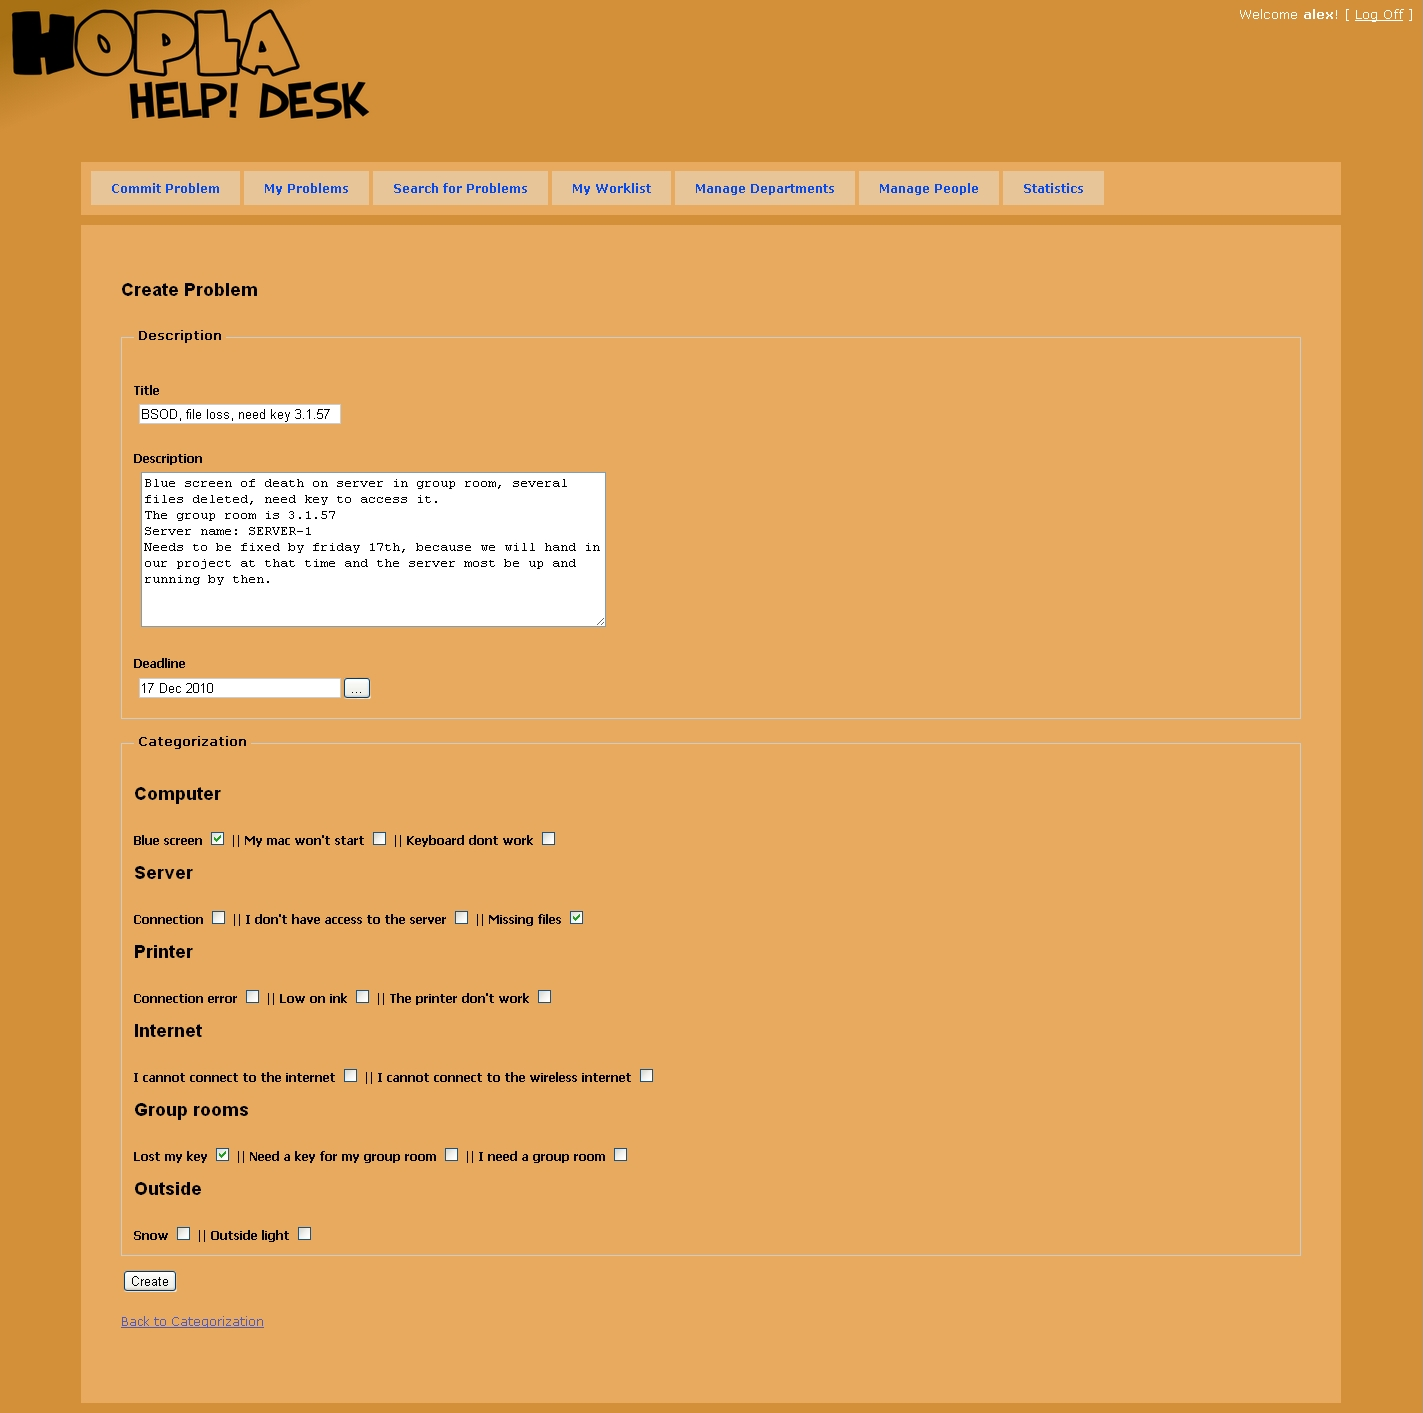
\includegraphics[width=1.00\textwidth, clip=true, trim=2.9cm 0.5cm 10cm 8cm]{input/implementation/program_presentation/newProblem.png}
	\morscaption{The create step of committing a new problem}
	\label{fig:newProblem}
\end{figure}
The \aclient[] can choose a problem(or even more problems) to subscribe to in order to receive notifications when the problem is updated, e.g. a solution is attached to it.
The \aclient[] can also choose to write a new problem if none of the existing problems suffice to match his/her problem.
The screen showed when creating a new problem is seen in figure \ref{fig:newProblem}

\subsection{See Own Problems}


\subsection{Search for Problems}